\documentclass{article}
\usepackage[margin=1.25in]{geometry}
\usepackage{amsmath, amssymb, setspace, enumerate, enumitem}
\usepackage{setspace}
\usepackage{graphicx}
\onehalfspacing

\begin{document}
    \begin{enumerate}
        \item \begin{enumerate}[label=(\alph*)]
            \item $k = 3$ was chosen as the optimal value for $k$, the graph is shown:\\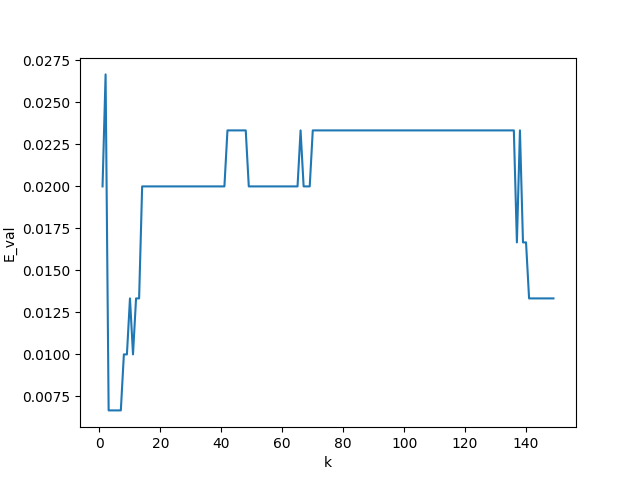
\includegraphics[scale=0.5]{images/1_a.png}
            \item For $k=3$, the decision boundary was:\\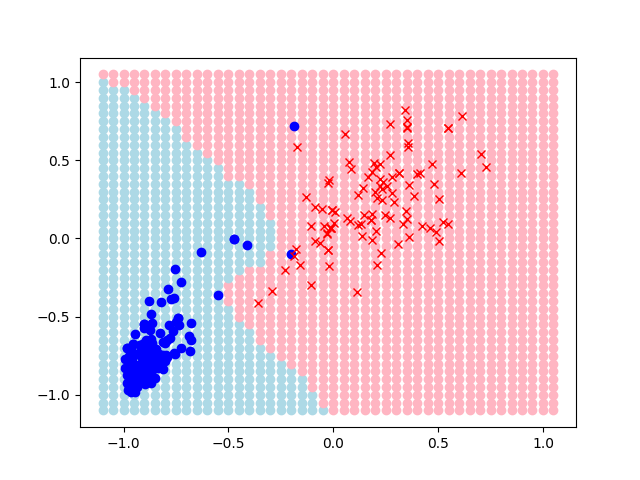
\includegraphics[scale=0.5]{images/1_b.png}\\My code uses in-sample error to choose the optimal $k$, so in sample and cross validation error were $0.0067$
            \item $0.0081$, test error was done by checking all the points in the validation set and comparing their output to what would've been the output in the training set.
        \end{enumerate}

        \item RBF network
    \end{enumerate}
\end{document}